% !TeX spellcheck = en_US
\begin{frame}
\Section{Solving Linear Systems with Iterative Methods}
\Subsection{Splitting Methods}
~\\
\textbf{Assumption} in this section: $A \in \Rnn$ is invertible, so that $x^* = A^{-1}b$ is the unique solution.\\~\\
%
\Subsubsection{Motivation and Overview}
%
\text{Problem:} \textit{The matrix $A$ can be very large} ($n \geq 10^5$)!\\
\begin{itemize}
	\item If $A$ can be stored, direct methods (such as LU, QR) are very slow or even not feasible due to large byproducts.
	\item Often $A$ cannot be stored, so that direct methods are not an option.
\end{itemize}
~\\~\\
Example:
\begin{itemize}
	\item A float with double precision (standard) needs 8 bytes of memory.\\\vspace{0.05cm}
	\item Considering 3d measurements with just 100 measurements in each dimension. \\
	$\Rightarrow$ $100 \cdot 100 \cdot 100 = 10^6$ measurements \\\vspace{0.05cm}
	\item Discretization methods (e.g., finite element method) for physical models (e.g., heat diffusion) interrelate these measurements. \\
	$\Rightarrow$ gives a matrix $A \in \Rnn$ with $n = 10^6$ \\	
	$\Rightarrow$ $n\cdot n = 10^{12}$ numbers have to be stored\\
	$\Rightarrow$ $10^{12}$ bytes $=$ $1$ \textbf{Terabyte} of memory has to be allocated in RAM {\bfseries\color{red}\LARGE $\lightning$}\\\vspace{0.05cm}
	\item A standard PC nowadays has 8--32 Gbytes of RAM (fast memory).
\end{itemize}
\end{frame}

\begin{frame}
	What if the matrix is \textit{sparse} (= many $0$ entries = redundancy)?\\
	$\rightarrow$ We only need to store nonzero entries and their coordinates (see, e.g., CSR from previous sheets).\\
	$\rightarrow$ \textbf{But:} Direct methods may still produce \textit{dense} ($\neq$ sparse) byproducts.\\
	\begin{center}
		{\color{black}
			\lstinputlisting[firstline=27,lastline=42]{media/NONZERO_count.py}
		}
		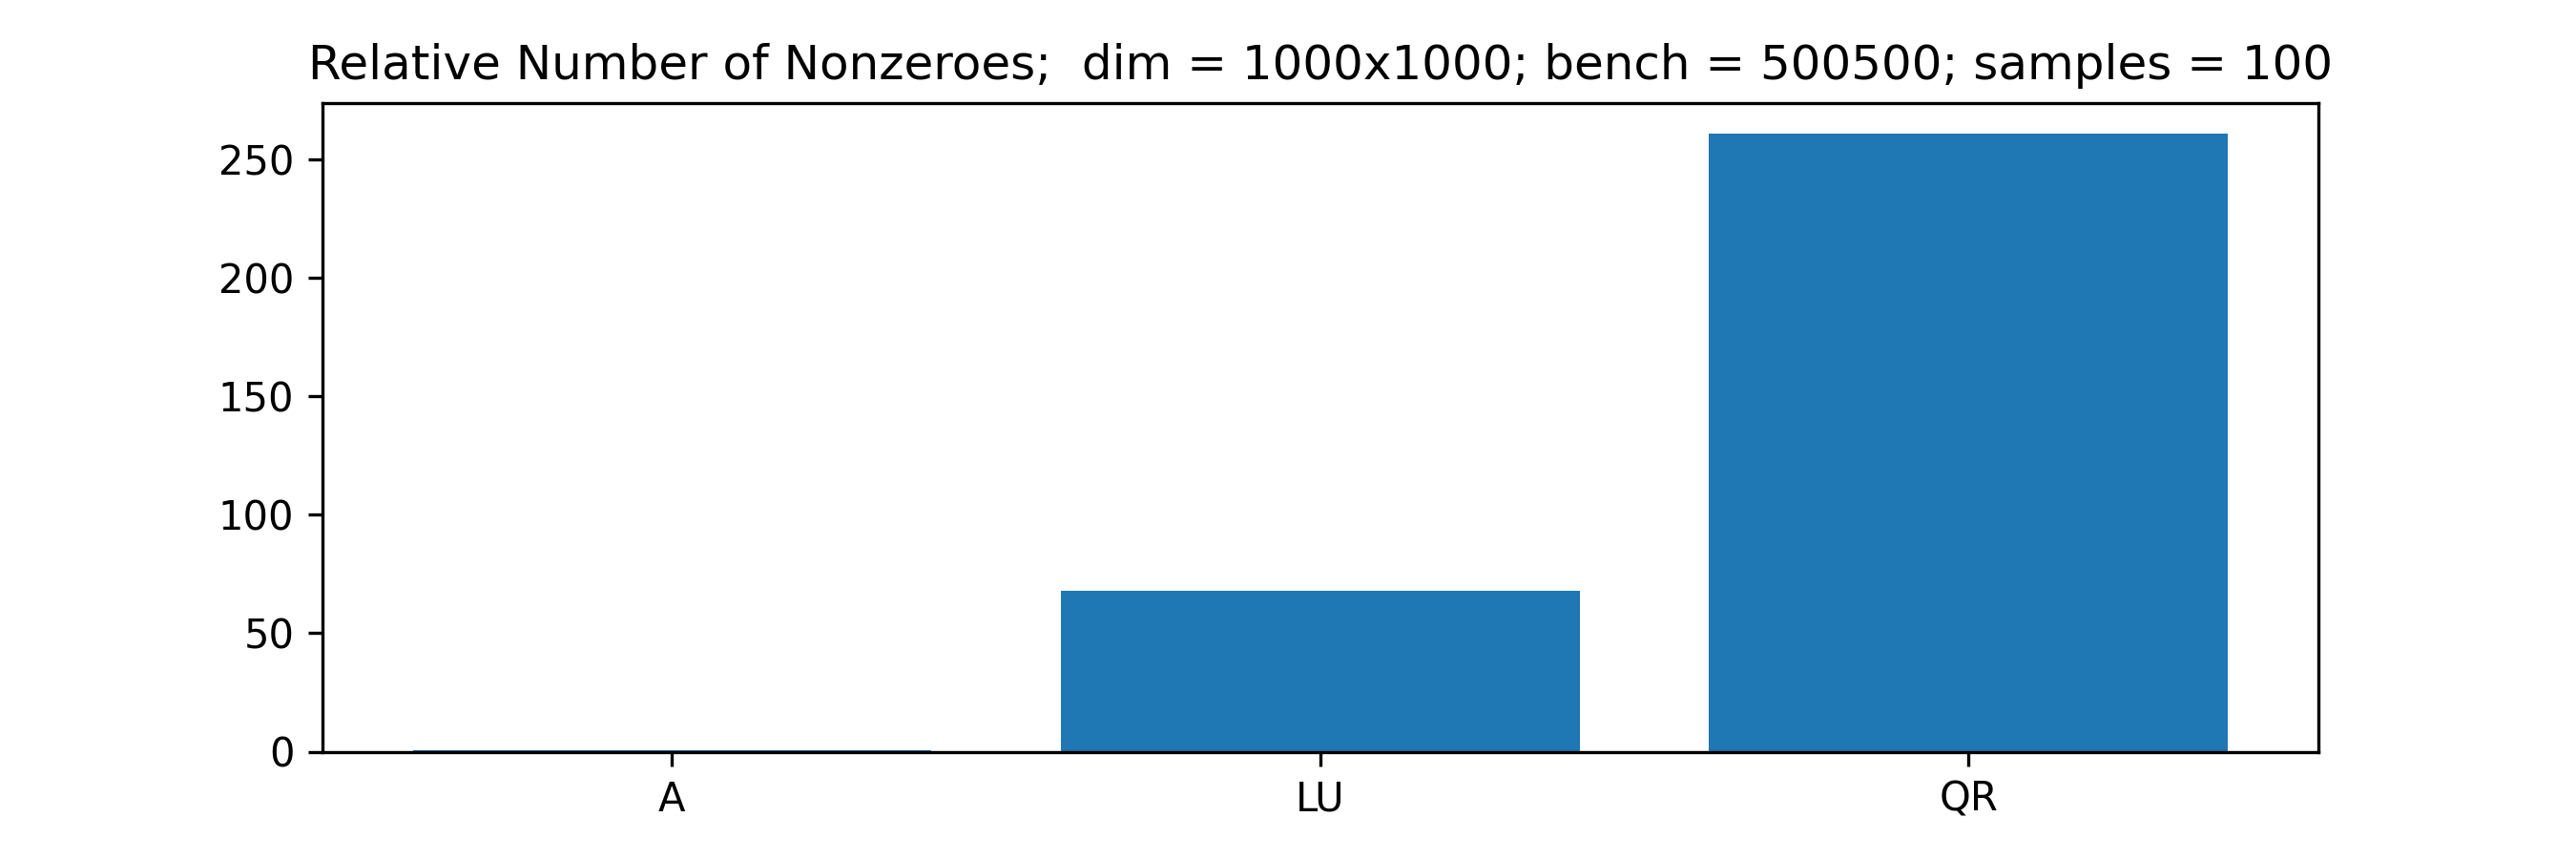
\includegraphics[width=0.6\textwidth]{NonzeroesInDirectMethods.png}
	\end{center} 
\end{frame}

\begin{frame}
~\\
\textbf{Key idea:} \textit{We do not need the full matrix, but only some matrix-vector product $x \mapsto S_Ax$}\\
~\\
 {\bf Approach:} Using this product we define a sequence $\{x^0,x^1,x^2,\ldots\}\subset\R^n$ such that
 \begin{itemize}
 	\item $x^k\to x^*\in\R^n$ for $k\to\infty$
 	\item $x^*$ solves the linear equation $Ax=b$
 	\item $x^{k+1}$ is a better approximation to $x^*$ than $x^k$
 \end{itemize} 
 ~\\~\\
 Standard classes of such iterations:\\
 \begin{itemize}
 \item[(1)] \textbf{Linear iterations (splitting methods)}  
 \item[(2)]  \textbf{Krylov subspace methods} 
\end{itemize}
 ~\\
\textbf{ Common advantages: }
 \begin{itemize}
 \item Even a few iteration steps may yield good results in stark contrast to LU (Gaussian Elimination), which has to be performed to the bitter end.~\\\vspace{0.2cm}
 \item The matrix $A$ or its decomposition does not need to be stored! Only a \textbf{matrix-vector product} $S_Ax$ has to be provided.~\\\vspace{0.2cm}
 \item In general, the overall computational complexity is lower than with \textit{direct} methods (LU, QR,...).~\\\vspace{0.2cm}
 \item[$\rightarrow$] Therefore: Iterative (=\textit{indirect}) methods are to be preferred, when the matrix is large (and sparse).
\end{itemize}
\end{frame}
 
 
\begin{frame}
~\\~\\
C.F. Gauß in a letter to Gerling from 1823\\ 
{\small (\url{https://gdz.sub.uni-goettingen.de/id/PPN23601515X?tify})}\\~\\~\\
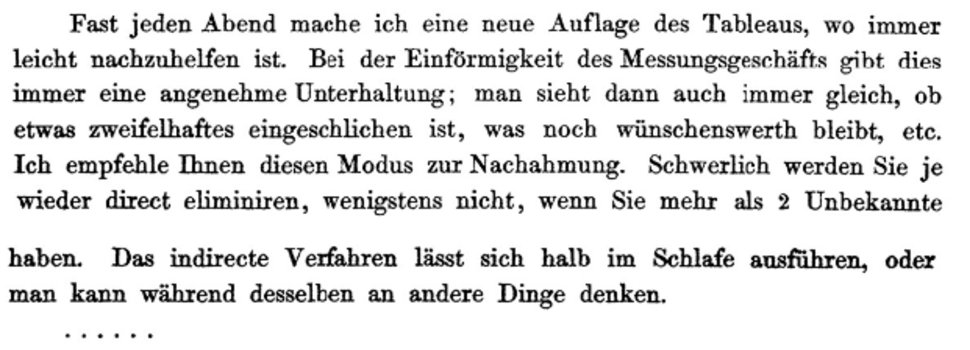
\includegraphics[width=0.8\textwidth]{gauss-seidel.pdf}
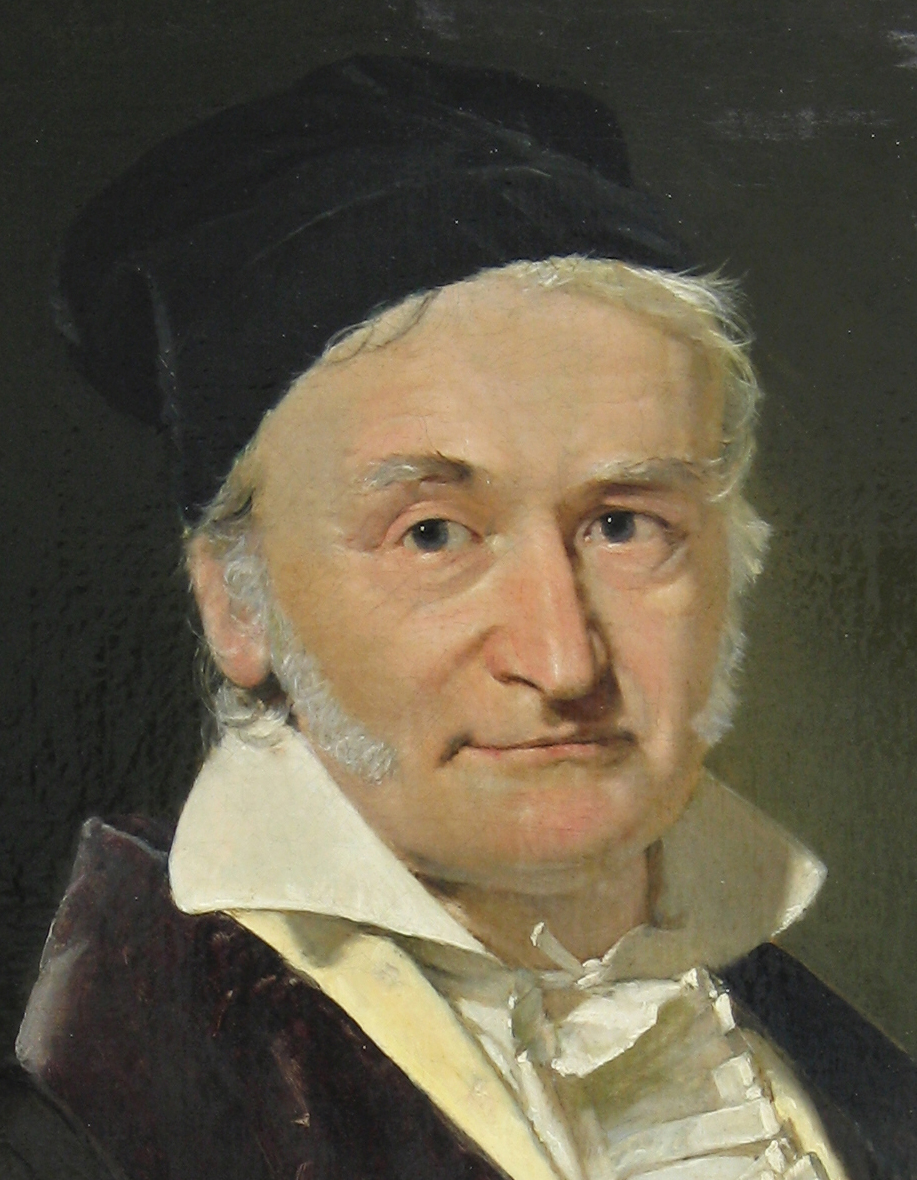
\includegraphics[width=0.2\textwidth]{Carl_Friedrich_Gauss.jpg}
~\\~\\
\begin{itemize}
	\item[$\rightarrow$] He already mentions an iterative method which was later coined \textit{Gauß-Seidel method}.\\
\item[$\rightarrow$] In general, one may need a lot of iteration steps but the aim is to keep the iteration instruction simple and fast.
\end{itemize}
\end{frame}
\begin{frame}
 \Subsubsection{A General Framework: Linear Fixed Point Iteration}
Linear iterations are of the form 
$$x^{k+1}=Mx^k+Nb$$
with $M,N\in\R^{n\times n}$. The matrix $M$
is called the \textbf{\color{defgruen}iteration matrix} and motivates the adjective ``linear''.\\[0.4cm]
 ~\\
We first derive a general convergence result and then relate $M$ and $N$ to the system $Ax=b$.\\~\\
\textbf{Convergence analysis}
\begin{defi}[Spectral radius]
	Let $M \in \R^{n\times n}$. Then the largest eigenvalue of $M$ in magnitude is called the \textbf{spectral radius of $M$} and denoted by $\rho(M)$, more precisely 
	$$\rho(M):=\max \{|\lambda_1|,\ldots, |\lambda_n|\}.$$
\end{defi}
~\\
\begin{theo}[Fixed point iteration] \label{theo:fixedpointiteration}
Let $M,N\in\R^{n\times n}$ and $b\in \R^n$. If $\rho(M)<1$, then the sequence $$x^{k+1}=Mx^k+Nb$$ converges for any starting point $x^0$ and its limit $x^* \in \R^n$ is a fixed point of the affine linear function $x\mapsto Mx+Nb$, i.e.,
$$ x^* = Mx^*+Nb.$$
\end{theo} \vspace{-0.5cm}
%\begin{proof} The proof needs the Jordan form (later).
%\end{proof}
\end{frame}

\begin{frame}
\textbf{Proof for the special case that $M$ is symmetric:}\\[0.1cm]
\small
	\Hide{
	Let us consider the eigenvalues of $M$
	$$|\lambda_n|\leq|\lambda_{n-1}|\leq\dots\leq|\lambda_1|=:\rho(M)<1.$$
	Since $M$ is assumed to be symmetric, we can apply the theorem on the eigendecomposition of symmetric matrices and find $Q\in\mathbb{R}^{n\times n}$ orthogonal, $\Lambda\in\mathbb{R}^{n\times n}$ diagonal, so that
	$$M=Q\Lambda Q^T,~\text{where}~~\Lambda=\begin{pmatrix}
	\lambda_1&~&0\\
	~&\ddots&~\\
	0&~&\lambda_n
	\end{pmatrix}.$$
	We will exploit two properties that we can conclude from $\rho(M)<1$. First, we observe that the powers of $M$ vanish. More precisely,
	\begin{align*}
	&M^2=M\cdot M=Q\Lambda\underbrace{Q^TQ}_{=I}\Lambda Q^T=Q\Lambda^2Q^T\\
	&\vdots\\
	&M^k=Q\Lambda^kQ^T=Q\begin{pmatrix}
	\lambda_1^k&~&0\\
	~&\ddots&~\\
	0&~&\lambda_n^k
	\end{pmatrix}
	Q^T\xrightarrow[(\rho(M)<1)]{k\rightarrow\infty}0.
	\end{align*}
	Secondly, we note that the so-called Neumann series converges: $\sum_{j=0}^\infty M^j=(I-M)^{-1}$ (general result, no proof here). Now we are in the position to proof the convergence result. Therefore let $x^0\in\mathbb{R}^n$, then
	\begin{align*}
	x^{k+1}=M\cdot\underbrace{x^k}_{{\color{cyan}=~Mx^{k-1}+Nb}}+Nb
	=\underbrace{M^kx^0}_{{\color{cyan}\xrightarrow{k\rightarrow\infty}0}}+\underbrace{\left(\sum_{j=0}^{k-1}M^j\right)}_{{\color{cyan}\xrightarrow{k\rightarrow\infty}(I-M)^{-1}}}\cdot Nb~
\xrightarrow{k\rightarrow\infty}~(I-M)^{-1}Nb=:x^*
 ~~\Leftrightarrow~~Nb=(I-M)x^* 
	\end{align*}
	Which is equivalent to
	$x^* = Mx^*+Nb$. Thus, the limit $x^*$ is a fixed point.
}
\end{frame}

\begin{frame}
\Subsubsection{Splitting Methods}
We now apply Theorem \ref{theo:fixedpointiteration} to the linear system $Ax=b$ by reformulating it as a fixed point problem. We also explain the idea of \textit{preconditioning}.\\
\Hide{
~\\
\textbf{General scheme: } $$x^{k+1}=Mx^k+Nb$$
\textbf{First Approach}\\
We rewrite the original system into a fixed point problem:
$$Ax=b~~\Leftrightarrow~~(x-x)+Ax=b~~\Leftrightarrow~~x=(I-A)x+Ib.$$
Then, if $\rho(I-A)<1$, we can conclude by Theorem \ref{theo:fixedpointiteration} that the fixed point iteration converges 
$$x^{k+1}=(I-A)x^k+b\xrightarrow{k\rightarrow\infty}x^* ,~~\text{with}~ Ax^*=b.$$
~\\
\textbf{Preconditioning}\\
We see that the success of this procedure relies on the condition $\rho(I-A)<1$. Unfortunately this is not generally the case, even not for invertible matrices (e.g., $A=2I \in \text{GL}_n(\R)$, then $\rho(I-A)=1$). An idea to increase our chances is to first \textit{precondition} the original system: Let $N\in\mathbb{R}^{n\times n}$ be invertible, then
\begin{align*}
Ax=b~~\Leftrightarrow~~\underbrace{NA}_{=:\tilde{A}}x=\underbrace{Nb}_{=:\tilde{b}}~~\Leftrightarrow~~\tilde{A}x=\tilde{b}~~\Leftrightarrow~x=(I-\tilde{A})x^k+\tilde{b}=(I-NA)x+Nb.
\end{align*}
Now for this preconditioned fixed point problem: If $\rho(I-NA)<1$, we can conclude by Theorem \ref{theo:fixedpointiteration} that the fixed point iteration converges 
$$x^{k+1}=(I-NA)x^k+Nb\xrightarrow{k\rightarrow\infty}x^* ,~~\text{with}~ Ax^*=b.$$
}
\end{frame}
 
\begin{frame}
\textbf{What is a good preconditioner?}\\~\\

\Hide{
	The optimal choice would be $N = A^{-1}$, because in this case we obtain the solution after one step:
	$$x^1=(I-NA)x^0+Nb=A^{-1}b.$$
	Access to the inverse would make our whole endeavor in this section dispensable. However, it serves as a compass to construct good preconditioners, which are mappings $x \mapsto Nx$ for which $N\approx A^{-1}$.\\~\\
%	 ~\\
%	\underline{Advantage:}\\
The advantage and aim of preconditioners are not only to higher our chances for convergence, but also to accelerate the convergence. In fact, by using a good preconditioner $N\approx A^{-1}$, we cannot only make sure that the convergence criteria
	$$
	\rho(I-\tilde{A})=\rho(I-NA)\ll 1
	$$
	is satisfied, but we can also show that the smaller $\rho(I-NA)$, the faster is the convergence.
}
\end{frame}

\begin{frame}
\textbf{How to construct a preconditioner?}
	\Hide{ 
\begin{itemize}
	\item Very simple preconditioning: \textbf{``Relaxation''}\\
	Often it already suffices to make the steps small enough. This idea corresponds to the preconditioner
	\begin{align*}
	N:=\theta I,~~\text{with sufficiently small~~} ~~0<\theta \begin{cases}
		=1:~&\text{no relaxation}\\
		<1:~&\text{relaxation}\\
		>1:~&\text{over-relaxation}
	\end{cases}
	\end{align*}
	The iteration matrix  is then given by
	$$M=I-\theta A.$$
~\\
	\item Next idea: \textbf{``Splitting based''}\\
	Recall that the best preconditioner is $N=A^{-1}$, which is not accessible. However, what about inverting just a (significant) part of $A$? In order to find such parts which are easy to invert, we consider the splitting of the matrix in the form:\\
	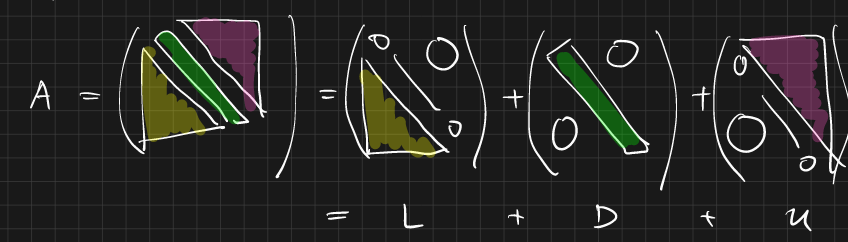
\includegraphics[width=0.6\textwidth]{LDU.png}~\\~\\
    For example, $D$ and $(L+D)$ are diagonal and lower triangular, respectively. Thus they are easy to invert (i.e., to solve for) and we may obtain $A^{-1}\approx D^{-1}$ or $A^{-1}\approx(L+D)^{-1}$, respectively.
\end{itemize}
}
\end{frame}

\begin{frame}
\textbf{\color{header}General scheme:}
\footnotesize
$$x^{k+1} = (I-NA)x^k + Nb = x^k - N(Ax^k-b)$$
%Desirable choice: $N \approx A^{-1}$
%~\\
%We consider the splitting $A = L + D + U$\\
~\\
\hspace*{-0.2cm}\begin{tabular}{l|l|l|l} 
\textbf{Preconditioner} 			& \textbf{Iteration Matrix} & \textbf{Iteration Instruction} & \textbf{Method Name}\\[0.25cm]
$N$ &$M=I - NA$& $x^{k+1} = x^k -N(Ax^k - b)$&\\[0.25cm]
\hline\\
%% RICH
${\color{cyan}\theta I}$ 	   		&$M_{Rich} =I-{\color{cyan}\theta} A$ 		&$x^{k+1}=x^k-\theta(Ax^k-b)$				& (relax.)\textbf{ Richardson}  \\[0.99cm]
%% JAC
${\color{cyan}\theta D^{-1}}$		&$M_{Jac} =  I-{\color{cyan}\theta D^{-1}}A$ 		&$x^{k+1}=x^k-\theta D^{-1}(Ax^k-b)$ 		&(weighted)\textbf{ Jacobi}\\[0.2cm]
%&&\textit{\footnotesize (where we assume: $a_{ii} \neq 0$)}& \\[0.2cm]
&$=(1-\theta)I-\theta D^{-1}(L+U)$&\textit{\footnotesize Element-based:}&\\
&& ${\color{orange}x^{k+1}_i = (1-\theta)x_i^k +  \frac{\theta}{a_{ii}}\left( b_i - \sum_{j\neq i} \,a_{ij} \, x_j^{k+1}\right)  }$ &\\[0.99cm]
%% GS
${\color{cyan}( L+D )^{-1}}$&$M_{GS} =I-{\color{cyan}( L+D )^{-1}}A$ 	&$x^{k+1}=x^k-( L+D )^{-1}(Ax^k-b)$  	&\textbf{Gauß-Seidel}\\[0.2cm]
%&&\textit{\footnotesize (where we assume: $a_{ii} \neq 0$)}&  \\[0.2cm]
&~~~$=(L+D)^{-1}U$&\textit{\footnotesize Element-based:}&\\
&& ${\color{orange}x^{k+1}_i =   \frac{1}{a_{ii}}\left( b_i - \sum\limits^{i-1}_{j=1} \,a_{ij} \, x_j^{k+1} -  \sum\limits^n_{j = i+1} \, a_{ij} \, x^k_j  \right) }$ &\\[0.99cm]
%% SOR
${\color{cyan}\theta( \theta L+D )^{-1}}$&$M_{SOR} =I-{\color{cyan}\theta( \theta L+D )^{-1}}A$ 	&$x^{k+1}=x^k-\theta( \theta L+D )^{-1}(Ax^k-b)$  	&\textbf{Successive Over--Relaxation (SOR)}\\[0.2cm]
&{\scriptsize $=(\theta L +D)^{-1} ((1-\theta)D-\theta U)$}&\textit{\footnotesize Element-based:}&\\
&& ${\color{orange}x^{k+1}_i = (1-\theta)x_i^k}$\\
&&~~~~~$ {\color{orange}+   \frac{\theta}{a_{ii}}\left( b_i - \sum\limits^{i-1}_{j=1} \,a_{ij} \, x_j^{k+1} -  \sum\limits^n_{j = i+1} \, a_{ij} \, x^k_j  \right) }$ &
\end{tabular}
\end{frame}





\begin{frame}
\textbf{\color{header}When does $\rho(M) <1$ hold?}~\\~\\

Idea: Derive some (possibly easy-to-compute) conditions which are sufficient for $\rho(M) <1$\\
$\rightarrow$ As usual, we often need to assume some properties for $A$ (e.g., symmetry).\\~\\
{
\small
\begin{tabular}{l|l}
\textbf{Method} & \textbf{Condition} \\
\hline \\
\textbf{(relax.) Richardson}& \underline{With relaxation ($\theta \neq 1$):}
\\
$M_{Rich} =I-{\color{cyan}\theta} A$	& If $A$ is symmetric and positive definite (spd), then:\\
&~~~~~~~~~~~~~~~~~~~~~~ $\rho(M_{Rich}) < 1 ~~\Leftrightarrow~~  0 < \theta < \frac{2}{\lambda_{max}(A)}$ \\
%optimal choice: $\theta_{opt} = \frac{2}{\lambda_{max}(A)+\lambda_{min}(A)}$\\
&\\[0.3cm]
\textbf{(weighted) Jacobi}& \underline{No relaxation ($\theta = 1$):}\\
$M_{Jac} =  I-{\color{cyan}\theta D^{-1}}A$&If $A$ is strictly diagonally dominant (i.e., $|a_{ii}| > \sum_{i\neq j} |a_{ij}|$), then $\rho(M_{Jac}) < 1$\\[0.3cm]
%	&{\footnotesize this is not a necessary condition: there are spd matrices for which the method diverges without relaxation}\\
& \underline{With relaxation ($\theta \neq 1$):}\\
&If $A$ is spd, then: \\
&~~~~~~~~~~~~~~~~~~~~~~   $\rho(M_{Jac}) < 1 ~~\Leftrightarrow~~  0 < \theta < \frac{2}{\lambda_{max}(D^{-1}A)}$\\[0.3cm]
& \\%optimal choice: $\theta_{opt} = \frac{2}{\lambda_{max}(D^{-1}A)+\lambda_{min}(D^{-1}A)}$\\
%% GAUß-SEIDEL
\textbf{Gauß-Seidel}& $\bullet$ If $A$ is strictly diagonally dominant, then $\rho(M_{GS}) < 1$\\
$M_{GS} =I-{\color{cyan}( L+D )^{-1}}A$& $\bullet$ If $A$ is spd, then $\rho(M_{GS}) < 1$\\[0.5cm]
%% SOR
\textbf{Successive Over--Relaxation (SOR)}& If $A$ is spd, then $\rho(M_{SOR}) < 1$ for $0 < \theta < {\bf2}$\\
$M_{SOR} =I-{\color{cyan}\theta( \theta L+D )^{-1}}A$ &\\
\end{tabular}
}
~\\\footnotesize ~\\
\textbf{Remark:} For many matrix classes (e.g., symmetric), we find 
$$\rho(M_{GS})\le \rho(M_{Jac}) \le \rho(M_{Rich})~~~~~~(\theta = 1).$$
%~\\~\\
%{\footnotesize
%	\blank
%	intuitively: $\theta$ small to assure small spectral radius\\
%	The spectral radius is a lower bound to any matrix norm derived from a vector norm.\\	
%	
%}

\end{frame}



\begin{frame}
	\textbf{Example}\\
	\Hide{\footnotesize
	Let us consider the symmetric tridiagonal matrix
	\begin{align*}
	A=\begin{pmatrix}
	3&-1&~&0\\
	-1&\ddots&\ddots&~\\
	~&\ddots&\ddots&-1\\
	0&~&-1&3
	\end{pmatrix}&=\begin{pmatrix}
	0&~&~&0\\
	-1&\ddots&~&~\\
	~&\ddots&\ddots&~\\
	0&~&-1&0
	\end{pmatrix}+\begin{pmatrix}
	3&~&0\\
	~&\ddots&~\\
	0&~&3
	\end{pmatrix}+\begin{pmatrix}
	0&-1&~&0\\
	~&\ddots&\ddots&~\\
	~&~&\ddots&-1\\
	0&~&~&0
	\end{pmatrix}\\
	&=~~~~~~~~~L~~~~~~~~~~~~~+~~~~~~~~~~D~~~~~~~~~~+~~~~~~~~~~~~U
	\end{align*}
	For large $n$ this matrix is extremely sparse:
	\begin{align*}
	&\frac{\sharp~\text{nonzero entries}}{n^2}=\frac{n+2(n-1)}{n^2}\xrightarrow{n\rightarrow\infty}0.
	\end{align*}
Based on the convergence criteria from the table above, we now check which methods would converge here. Since $|3|>|-1|+|-1|$ it is easily verified that $A$ is strictly diagonally dominant. Therefore Jacobi and Gauß-Seidel converge.\\~\\
What about the Richardson method? For simplicity we consider $n=3$ and compute the eigenvalues of $A$ and find
\begin{align*}
\text{det}(A-\lambda I)=\text{det}\begin{pmatrix}
3-\lambda&-1&0\\
-1&3-\lambda&-1\\
0&-1&3-\lambda
\end{pmatrix}&\\
\stackrel{\text{Sarrus}}{=} -(3-\lambda)^3+ ( 3-\lambda)+(3-\lambda)&\\
= (3-\lambda) \cdot (2-(3-\lambda)^2) \stackrel{!}{=}0
&\Leftrightarrow~~ \lambda=3,~(3-\lambda)=\pm\sqrt{2}~~\Leftrightarrow~~\lambda=3,~\lambda=3\pm\sqrt{2} 
\end{align*}
Since all eigenvalues of this symmetric matrix are positive, we have that $A$ is positive definite. Noting that $\lambda_{max}(A)=3+\sqrt{2}$, we apply the above convergence criteria and find that the relaxed Richardson method converges, if the the relaxation parameter is chosen from the interval $$0 < \theta < \frac{2}{\lambda_{max}(A)}=\frac{2}{3+\sqrt{2}} \approx 0.45 < 1.$$
}
\end{frame}
\begin{frame}
\textbf{Final Remarks}
	\begin{itemize}
		\item Using the Richardson iteration we only need the evaluation of the matrix vector product $x \mapsto Ax$ to solve the system $Ax=b$.
		\item All iterations of the form $x^{k+1}= x^k - N(Ax^k-b)$ can be seen as preconditioned Richardson iterations. Next semester you will learn a strong correspondence between the Richardson method and the gradient method, as well as preconditioned Richardson method and Newton-type methods to minimize functions of the form $f(x):=\frac{1}{2}x^\top Ax-b^\top x$.
		\item By looking at the element-wise formulas for the Jacobi (with $\theta = 1$) and Gauß-Seidel method (see the orange formulas in the table above) we can understand these methods as alternating methods. Consider for example the simple case $n=2$ and write out these formulas. Then you will see that we alternatingly compute the components $x_1$ and $x_2$.
		\item Similar to a block LU factorization, we can consider blocks $A_{ij}$ (= matrices) instead of numbers $a_{ij}$ in the element-wise formulas of Jacobi and Gauß-Seidel. Thereby, one obtains the block Jacobi and block Gauß-Seidel method. These are highly related to so called additive and multiplicative Schwarz methods, respectively.
		\item In practice, splitting methods (or more precisely the preconditioner $N$) are mainly used as preconditioners for Krylov subspace methods, which we will address in the next section.
	\end{itemize}
\end{frame}







%PAGERANK example
%\begin{frame}
%{\bf PageRank example:}$$x^{k+1}:=\alpha Px^{k}+(1-\alpha)v$$ for the linear PageRank system $(I-\alpha P)x=(1-\alpha)v$ is a Richardson iteration for \\ 
%$A=I-\alpha P,~~ b=(1-\alpha)v,~~ \theta=1, N = I$\\
%In fact, we find
%\[
%x^{k+1}=x^k-\theta(Ax^k-b)=x^k-((I-\alpha P)x^k-(1-\alpha)v) = \alpha Px^{k}+(1-\alpha)v
%\]
%Does it converge? $\rightarrow$ we have to check the spectral radius of $M=(I-NA)=\alpha P$, where $P$ is column stochastic.
%\rbegin{lemma}
%The spectral radius of a stochastic matrix is less or equal than one. 
%\bend{lemma}
%\vspace{-0.5cm}
%\begin{proof}
%	\blank
%	A column (row) stochastic matrix $P$ has the property that each column (row) contains nonnegative entries, which add up to 1. From the characterization of eigenvalues via roots of a polynomial in theorem \ref{eigenpoly}, we observe that $\sigma(P^\top)=\sigma(P)$. Thus, without loss of generality, let us consider an eigenvalue $\lambda\in\sigma(P)$ of a row stochastic matrix $P$, with corresponding eigenvector $v$. 
%	Define the index $\ell$ by $|v_\ell|=\max\{|v_1|,\ldots,|v_n|\}\neq 0$. Then
%	\begin{align*}
%	|\lambda|\cdot |v_\ell|&=|a_{\ell ,1}v_1+\ldots+a_{\ell,n}v_n|\le |a_{\ell ,1}||v_1|+\ldots+|a_{\ell,n}||v_n|\\
%	&\le |a_{\ell ,1}||v_\ell|+\ldots+|a_{\ell,n}||v_\ell|=(a_{\ell ,1}+\ldots+a_{\ell,n})|v_\ell|=|v_\ell|
%	\end{align*}
%\end{proof}
%Therefore $\rho(P)\le 1$ and if $0<\alpha<1$ we find $\rho(\alpha P)<1$. Thus, we have shown convergence.
%\end{frame}